\question \textbf{UPGMA}

UPGMA is an unweighted version of PGMA (pair-group method using arithmetic mean) for reconstructing a phylogenetic tree. Pairwise sequence alignments are used to calculate the distances among four sequences A, B, C, and D.

\begin{table}[H]
\centering
\begin{tabular}{lllll}
                       & A                      & B                      & C                      & D                      \\ \cline{2-5} 
\multicolumn{1}{l|}{A} & \multicolumn{1}{l|}{0} & \multicolumn{1}{l|}{2} & \multicolumn{1}{l|}{7} & \multicolumn{1}{l|}{7} \\ \cline{2-5} 
B                      & \multicolumn{1}{l|}{}  & \multicolumn{1}{l|}{0} & \multicolumn{1}{l|}{5} & \multicolumn{1}{l|}{9} \\ \cline{3-5} 
C                      &                        & \multicolumn{1}{l|}{}  & \multicolumn{1}{l|}{0} & \multicolumn{1}{l|}{8} \\ \cline{4-5} 
D                      &                        &                        & \multicolumn{1}{l|}{}  & \multicolumn{1}{l|}{0} \\ \cline{5-5} 
\end{tabular}
\end{table}

Below are two examples of the distance calculation that can be used for UPGMA.

\[
d_{(\alpha\beta),\gamma}=\dfrac{d_{\alpha,\gamma} + d_{\beta,\gamma}}{2}, \quad d_{(\alpha\beta\gamma),\delta}=\dfrac{d_{\alpha,\delta} + d_{\beta,\gamma} + d_{\delta,\gamma}}{3}
\]

\begin{parts}

\vspace{0.1 in}

%% (a)
  \part Identify the first internal node and update the distance matrix.
  
\begin{table}[H]
\centering
\begin{tabular}{
>{\columncolor[HTML]{CCE5FF}}c 
>{\columncolor[HTML]{CCE5FF}}c 
>{\columncolor[HTML]{CCE5FF}}c 
>{\columncolor[HTML]{CCE5FF}}c }
{\color[HTML]{000000} }                                                  & {\color[HTML]{000000} (AB)}                                           & {\color[HTML]{000000} C}                                              & {\color[HTML]{000000} D}                                              \\ \cline{2-4} 
\multicolumn{1}{c|}{\cellcolor[HTML]{CCE5FF}{\color[HTML]{000000} (AB)}} & \multicolumn{1}{c|}{\cellcolor[HTML]{CCE5FF}{\color[HTML]{000000} 0}} & \multicolumn{1}{c|}{\cellcolor[HTML]{CCE5FF}{\color[HTML]{000000} 6}} & \multicolumn{1}{c|}{\cellcolor[HTML]{CCE5FF}{\color[HTML]{000000} 8}} \\ \cline{2-4} 
{\color[HTML]{000000} C}                                                 & \multicolumn{1}{c|}{\cellcolor[HTML]{CCE5FF}{\color[HTML]{000000} }}  & \multicolumn{1}{c|}{\cellcolor[HTML]{CCE5FF}{\color[HTML]{000000} 0}} & \multicolumn{1}{c|}{\cellcolor[HTML]{CCE5FF}{\color[HTML]{000000} 8}} \\ \cline{3-4} 
{\color[HTML]{000000} D}                                                 & {\color[HTML]{000000} }                                               & \multicolumn{1}{c|}{\cellcolor[HTML]{CCE5FF}{\color[HTML]{000000} }}  & \multicolumn{1}{c|}{\cellcolor[HTML]{CCE5FF}{\color[HTML]{000000} 0}} \\ \cline{4-4} 
\end{tabular}
\end{table}

%% (b)
  \part Identify the second internal node and update the distance matrix accordingly.
  
\begin{table}[H]
\centering
\begin{tabular}{
>{\columncolor[HTML]{CCE5FF}}c 
>{\columncolor[HTML]{CCE5FF}}c 
>{\columncolor[HTML]{CCE5FF}}c }
{\color[HTML]{333333} }                                                   & {\color[HTML]{333333} (ABC)}                                          & {\color[HTML]{333333} D}                                              \\ \cline{2-3} 
\multicolumn{1}{c|}{\cellcolor[HTML]{CCE5FF}{\color[HTML]{333333} (ABC)}} & \multicolumn{1}{c|}{\cellcolor[HTML]{CCE5FF}{\color[HTML]{333333} 0}} & \multicolumn{1}{c|}{\cellcolor[HTML]{CCE5FF}{\color[HTML]{333333} 8}} \\ \cline{2-3} 
{\color[HTML]{333333} D}                                                  & \multicolumn{1}{c|}{\cellcolor[HTML]{CCE5FF}{\color[HTML]{333333} }}  & \multicolumn{1}{c|}{\cellcolor[HTML]{CCE5FF}{\color[HTML]{333333} 0}} \\ \cline{3-3} 
\end{tabular}
\end{table}

%% (c)
  \part Reconstrut a rooted tree from the calcualted distances.
  
\begin{figure}[H]
      \centering
      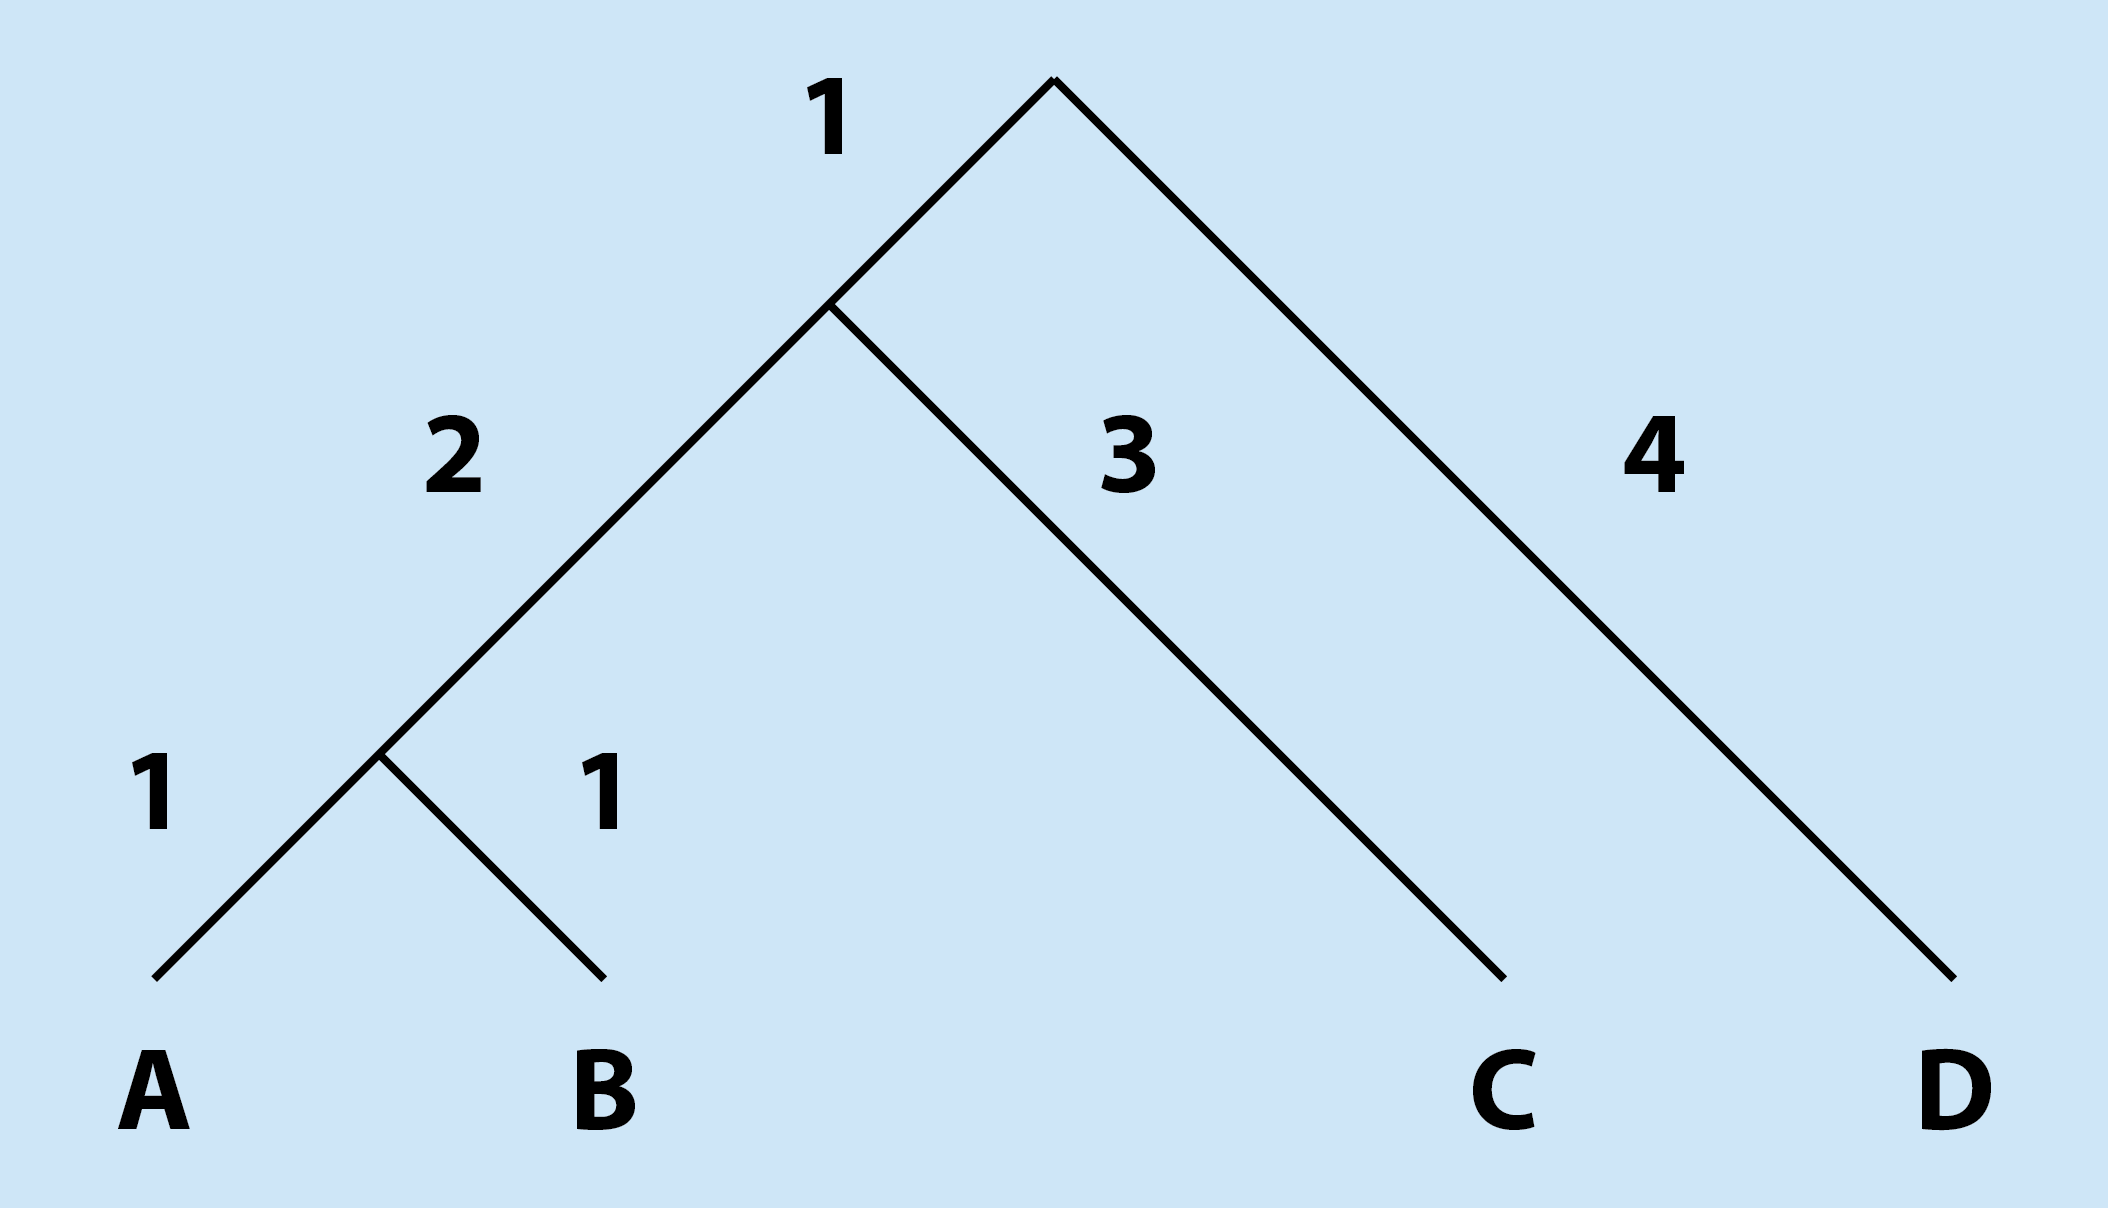
\includegraphics[width=0.3 \textwidth]{fig09/ultrametric_tree_solution.png}
\end{figure}
  
%% (d)
  \part Reconstruct a rooted tree by using UPGMA.
  
\begin{table}[H]
\centering
\begin{tabular}{lllll}
                       & A                      & B                                              & C                                              & D                                              \\ \cline{2-5} 
\multicolumn{1}{l|}{A} & \multicolumn{1}{l|}{0} & \multicolumn{1}{l|}{\cellcolor[HTML]{CCE5FF}2} & \multicolumn{1}{l|}{\cellcolor[HTML]{CCE5FF}6} & \multicolumn{1}{l|}{\cellcolor[HTML]{CCE5FF}8} \\ \cline{2-5} 
B                      & \multicolumn{1}{l|}{}  & \multicolumn{1}{l|}{0}                         & \multicolumn{1}{l|}{\cellcolor[HTML]{CCE5FF}6} & \multicolumn{1}{l|}{\cellcolor[HTML]{CCE5FF}8} \\ \cline{3-5} 
C                      &                        & \multicolumn{1}{l|}{}                          & \multicolumn{1}{l|}{0}                         & \multicolumn{1}{l|}{\cellcolor[HTML]{CCE5FF}8} \\ \cline{4-5} 
D                      &                        &                                                & \multicolumn{1}{l|}{}                          & \multicolumn{1}{l|}{0}                         \\ \cline{5-5} 
\end{tabular}
\end{table}

\end{parts}

